% Section content template for individual Educative lessons
% This file contains the actual content for a specific section
% Generated from Educative API section content

% Section: Concurrency in Collaborative Editing
% Section ID: 6200295243120640
% Section Slug: concurrency-in-collaborative-editing
% Generated: 2025-12-08T15:23:27.832361

\subsection{Introduction}\label{JI7_JXUu55toQ9-ba-sWu}
\\
We've discussed the design for a collaborative document editing service, but we haven't addressed how we'll deal with concurrent changes in the document by different users. However, before discussing concurrency issues, we need to understand the collaborative text editor.

\subsection{What is a document editor?}\label{Em6v51MakGgM2tvW5a68E}
\\
A \textbf{document} is a composition of characters in a specific order. Each character has a value and a positional index. The character can be a letter, a number, an enter (↵), or a space. An index represents the character's position within the ordered list of characters.
\\
The job of the text or document editor is to perform operations like \texttt{insert()}, \texttt{delete()}, \texttt{edit()}, and more on the characters within the document. A depiction of a document and how the editor will perform these operations is below.

\begin{figure}[htbp]
 \centering
 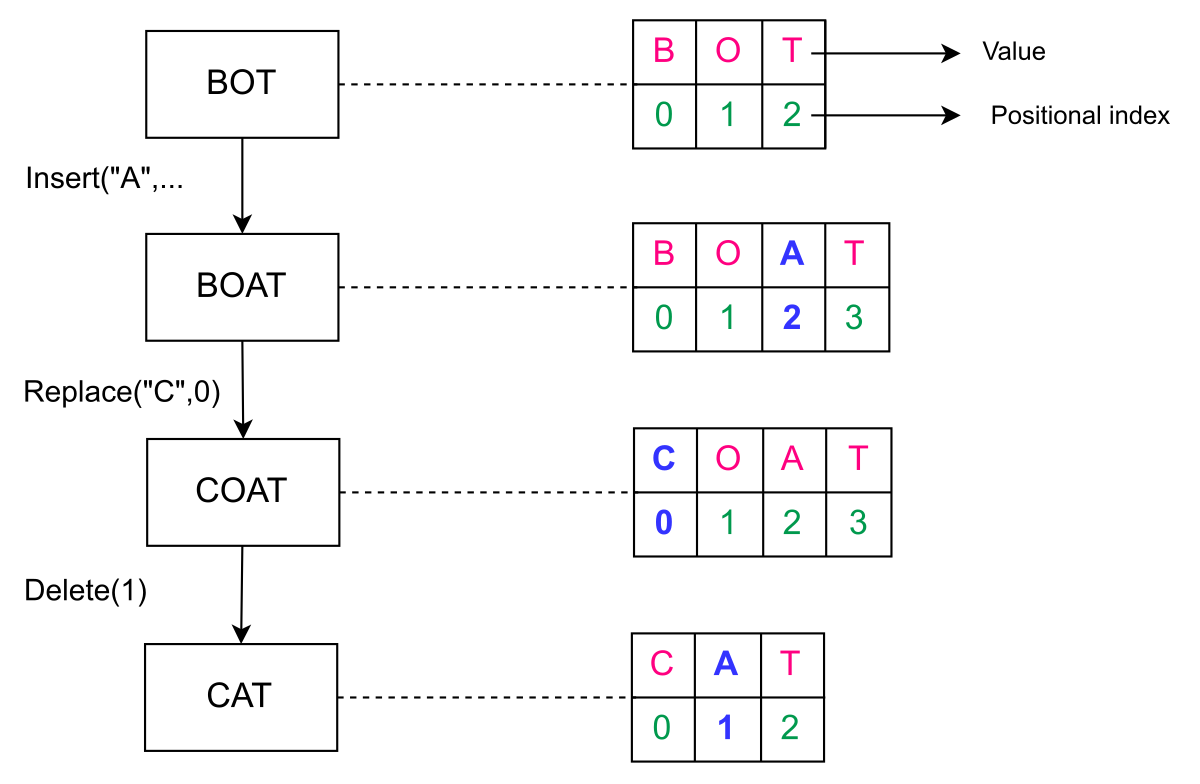
\includegraphics[width=0.5\textwidth]{Images/chapter_38/section_6200295243120640/5683325523460096.png}
 \caption{How a document editor performs different operations}
\end{figure}

\subsection{Concurrency issues}\label{t_0UCtAruaNDLRPEKLpMu}
\\
Collaboration on the same document by different users can lead to concurrency issues. Conflicts may arise whenever multiple users edit the same portion of a document. Since users have a local copy of the document, the final status of the document may be different at the server from what the users see at their end. After the server pushes the updated version, users discover the unexpected outcome.

\subsubsection{Example 1}\label{Lv2Qm-2u8bUraQ70bv5zI}
\\
Let's consider a scenario where two users want to add some characters at the same positional index. Below , we've depicted how two users modifying the same sentence can lead to conflicting results:

\begin{figure}[htbp]
 \centering
 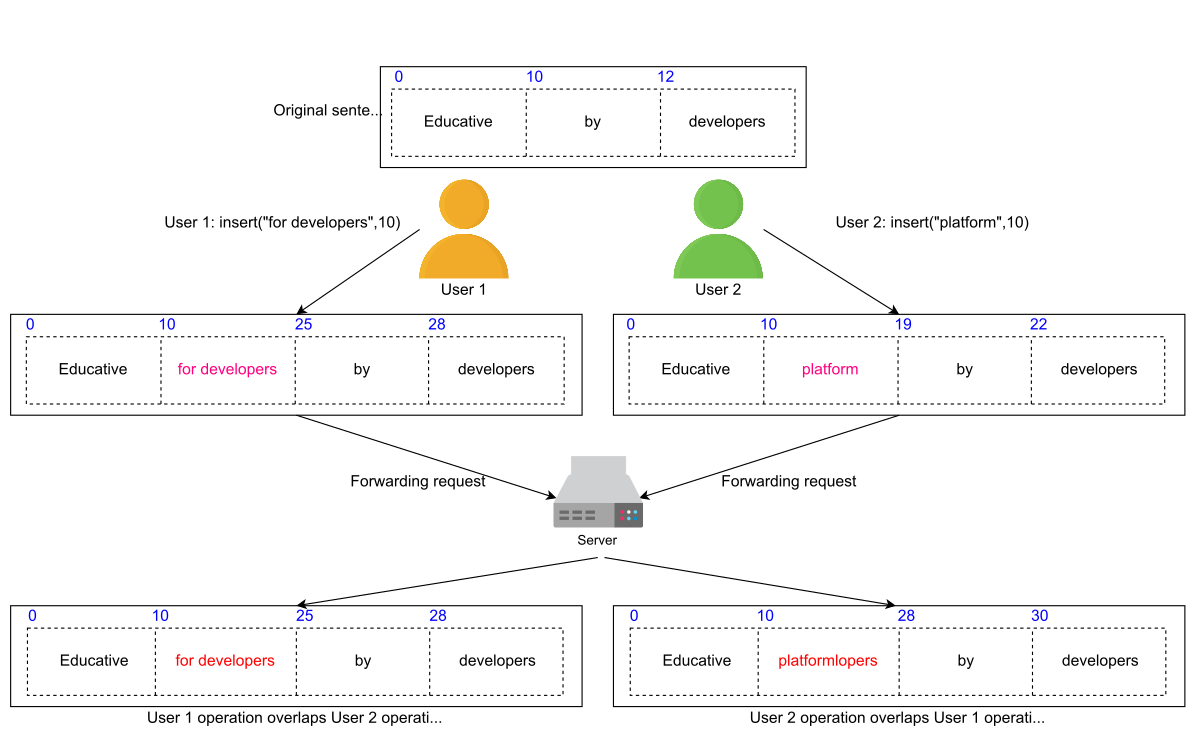
\includegraphics[width=0.5\textwidth]{Images/chapter_38/section_6200295243120640/6266785069793280.png}
 \caption{How two users modifying the same text can lead to concurrency issues}
\end{figure}

As shown above, two users are trying to modify the same sentence, ``Educative by developers.'' Both users are performing \texttt{insert()} at index \texttt{10}. The two possibilities are as follows:

\begin{itemize}
\item
\protect\phantomsection\label{_ocO7aIc-CQviQZYbhRH1}
The phrase ``for developers'' overwrites ``platform.'' This leads to an outcome of ``for developers.''
\item
\protect\phantomsection\label{jpr8NgFw9D_B0yoSB6IFZ}
The phrase ``platform'' overlaps ``for developers.'' This leads to an outcome of ``platformlopers.''
\end{itemize}
\\
This example shows that operations applied in a different order don't hold the commutative property.

\subsubsection{Example 2}\label{9-tD6jLdnN61SIqZrqVNQ}
\\
Let's look at another simple example where two users are trying to delete the same character from a word. Let 's use the word ``EEDUCATIVE.'' Because the word has an extra ``E,'' both the users would want to remove the extra character. Below
, we see how an unexpected result can occur:

\begin{figure}[htbp]
 \centering
 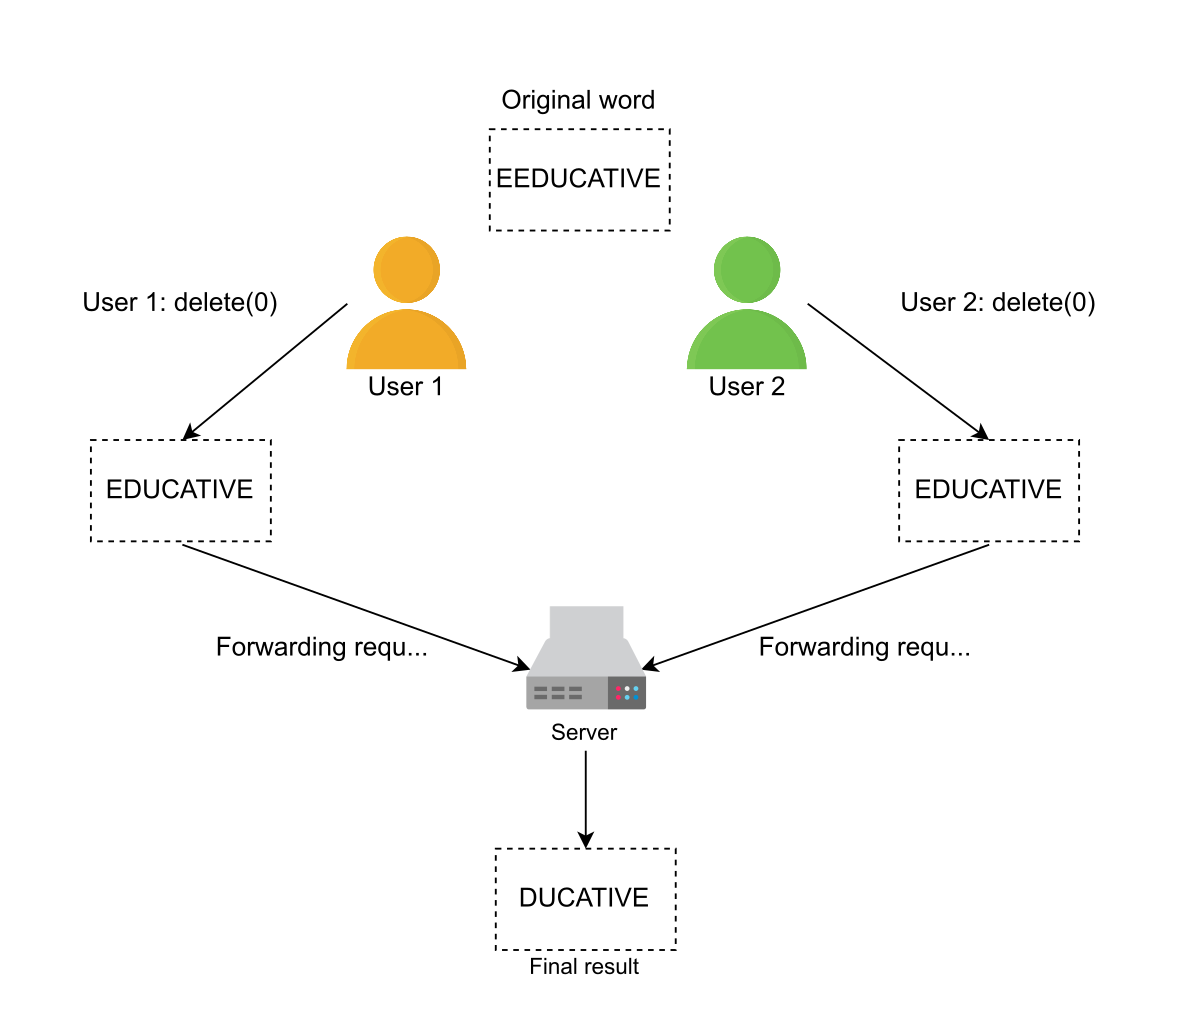
\includegraphics[width=0.5\textwidth]{Images/chapter_38/section_6200295243120640/6692955658387456.png}
 \caption{How deleting the same character can lead to unexpected changes}
\end{figure}

This second example shows that different users applying the same operation won't be idempotent(An operation with the same input produces the same results no matter how many times an operation repeats.). So , conflict resolution is necessary where multiple collaborators are editing the same portion of the document at the same time.
\\
From the examples above, we understand that a solution to concurrency issues in collaborative editing should respect two rules:

\begin{itemize}
\item
\protect\phantomsection\label{ixj5aOURZ6BWlSWa0MjQU}
\textbf{Commutativity}: The order of applied operations shouldn't affect the end result.
\item
\protect\phantomsection\label{NxMd-hWJkVCuyhr3qQNgF}
\textbf{Idempotency}: Similar operations that have been repeated should apply only once.
\end{itemize}
\\
Below, we identify two well-known techniques for conflict resolution.

\subsection{Techniques for conflict resolution}\label{ZAIes0X1IuL9UOLsSBv-j}
\\
Let's discuss two leading technologies that are used for conflict resolution in collaborative editing.

\subsubsection{Operational transformation}\label{2BV2KuaF_FvdaMzgvP2MA}
\\
\textbf{Operational transformation (OT)} is a technique that's widely used for conflict resolution in collaborative editing. OT emerged in 1989 and has improved throughout the years. It's a lock-free and non-blocking approach for conflict resolution. If operations between collaborators conflict, OT resolves conflicts and pushes the correct converged state to end users. As a result, OT provides consistency for users.
\\
OT performs operations using the positional index method to resolve conflicts, such as the ones we discussed above. OT resolves the problems above by holding commutativity and idempotency.

\begin{figure}[htbp]
 \centering
 \begin{subfigure}[b]{0.48\textwidth}
 \centering
 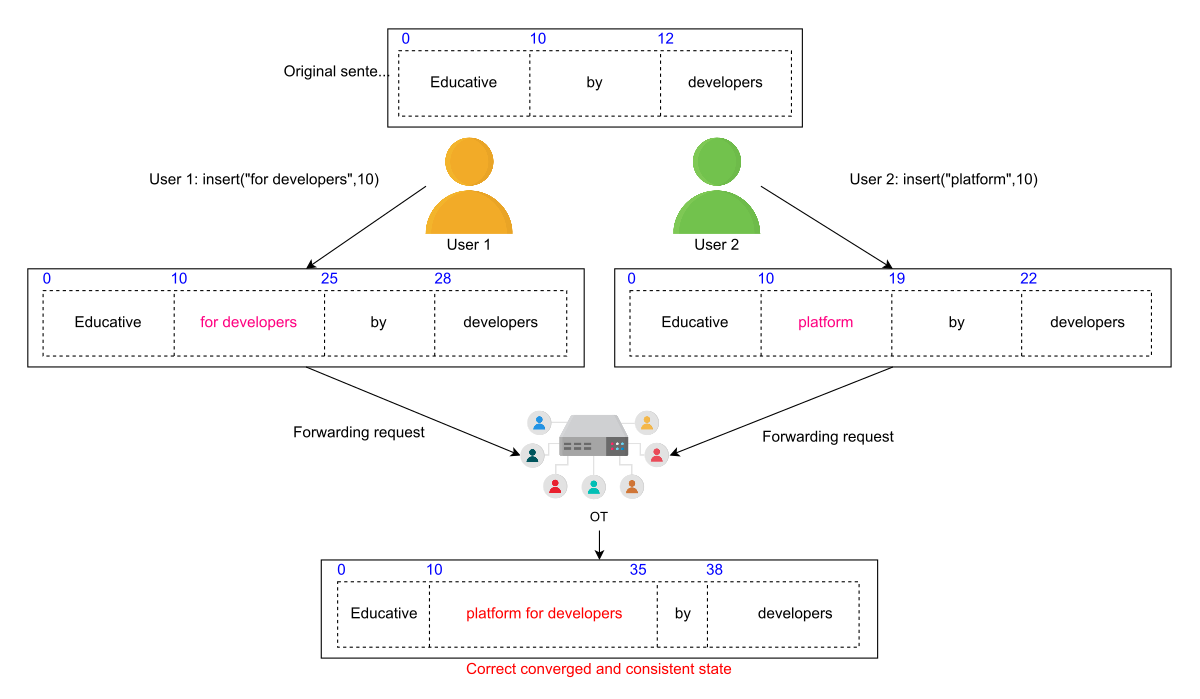
\includegraphics[width=\textwidth]{Images/chapter_38/section_6200295243120640/6741792951369728.png}
 \caption{Ensuring commutativity}
 \end{subfigure}
 \hfill
 \begin{subfigure}[b]{0.48\textwidth}
 \centering
 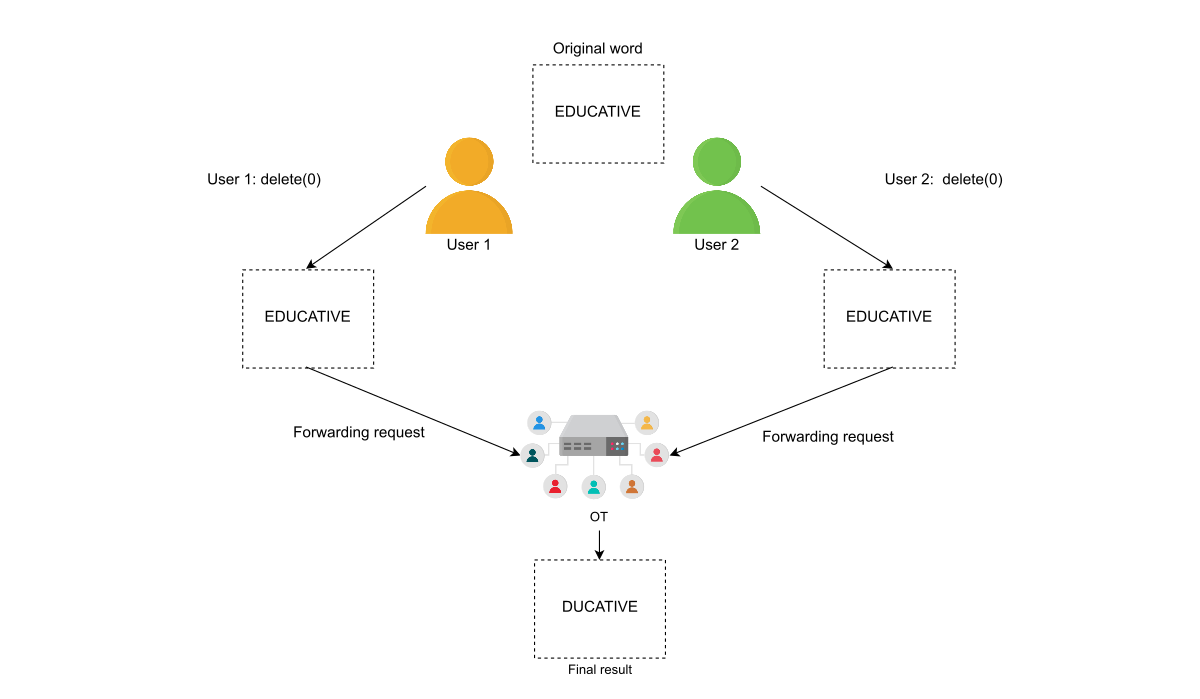
\includegraphics[width=\textwidth]{Images/chapter_38/section_6200295243120640/5861001311420416.png}
 \caption{Ensuring idempotency}
 \end{subfigure}
\end{figure}

Collaborative editors based on OT are consistent if they have the following two properties:

\begin{itemize}
\item
\protect\phantomsection\label{6J2W0HQeIjtGxqpABTopm}
\textbf{Causality preservation}: If operation \texttt{a} happened before operation \texttt{b}, then operation \texttt{a} is executed before operation \texttt{b}.
\item
\protect\phantomsection\label{DgY5Z2OVVujAPT_cXY392}
\textbf{Convergence}: All document replicas at different clients will eventually be identical.
\end{itemize}
\\
The properties above are a part of the \textbf{CC consistency model}, which is a model for consistency maintenance in collaborative editing.

The research community has proposed various consistency models over the years. Some of them are specific to collaborative editing, while others are specific to OT algorithms. The key consistency models are the following: * CC model: As we defined above, this includes causality preservation and convergence. * CCI model: This includes \#key\# causality preservation: Same as CC model. \#key\#, \#key\# convergence: Same as CC model. \#key\#, and \#key\# intention preservation: This property ensures that operations are executed as intended by the users. \#key\#.
\\
Other models include the CSM (\textbf{c} ausality, \textbf{s} ingle-operation effects, and \textbf{m} ulti-operation effects) model and the CA (\textbf{c} ausality and \textbf{a} dmissibility) model.
\\
Various consistency models are suggested, and usually, the newer ones are supersets of the earlier ones. Because there are so many proposed algorithms, discussing them is beyond the scope of our lesson. Interested readers can find more details \href{https://dl.acm.org/doi/pdf/10.1145/289444.289469}{here}.

OT has two disadvantages:

\begin{itemize}
\item
\protect\phantomsection\label{AAdxsuJ2sIQBxAqGSMUXD}
Each operation on characters may require changes to the positional index. This means that operations are order dependentorderDependent on each other.
\item
\protect\phantomsection\label{aN0EyXL_kcaOIzl_SlCyO}
It's challenging to develop and implement.
\end{itemize}
\\
Operational transformation is a set of complex algorithms, and its correct implementation has proved challenging for real-world applications. For example, the Google Wave team took two years to implement an OT algorithm.

\subsubsection{Conflict-free Replicated Data Type (CRDT)}\label{BZ2jsYA524p_Y9gChrHxr}
\\
The \textbf{Conflict-free Replicated Data Type (CRDT)} was developed in an effort to improve OT. A CRDT has a complex data structure but a simplified algorithm.
\\
A CRDT satisfies both commutativity and idempotency by assigning two key properties to each character:

\begin{itemize}
\item
\protect\phantomsection\label{VehxyltvNHB7YGyVfoieP}
It assigns a globally unique identity to each character.
\item
\protect\phantomsection\label{Uw9Dvd2PP6nN5UXsI5kCB}
It globally orders each character.
\end{itemize}
\\
Each operation now has an updated data structure:

\begin{figure}[htbp]
 \centering
 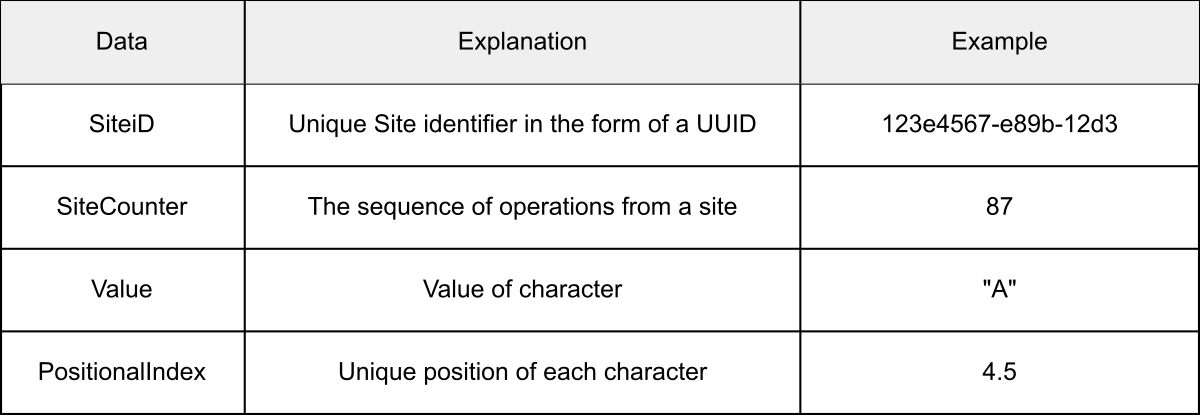
\includegraphics[width=0.5\textwidth]{Images/chapter_38/section_6200295243120640/5126789348720640.png}
 \caption{Simplified data structure of a CRDT}
\end{figure}

The \texttt{SiteID} uniquely identifies a user's site requesting an operation with a \texttt{Value} and a \texttt{PositionalIndex}. The value of \texttt{PositionalIndex} can be in fractions for two main reasons.

\begin{itemize}
\item
\protect\phantomsection\label{c3V3pkD5Y42nxYBMmGFuf}
The \texttt{PositionalIndex} of other characters won't change because of certain operations.
\item
\protect\phantomsection\label{ev5FMVqAsFeuPRiwoYO62}
The order dependency of operations between different users will be avoided.
\end{itemize}
\\
The example below depicts that a user from site ID \texttt{123e4567-e89b-12d3} is inserting a character with a value of \texttt{A} at a \texttt{PositionalIndex} of \texttt{1.5}. Although a new character is added, the positional indexes of existing characters are preserved using fractional indices. Therefore, the order dependency between operations is avoided. As shown below, an \texttt{insert()} between \texttt{O} and \texttt{T} didn't affect the position of \texttt{T}.

\begin{figure}[htbp]
 \centering
 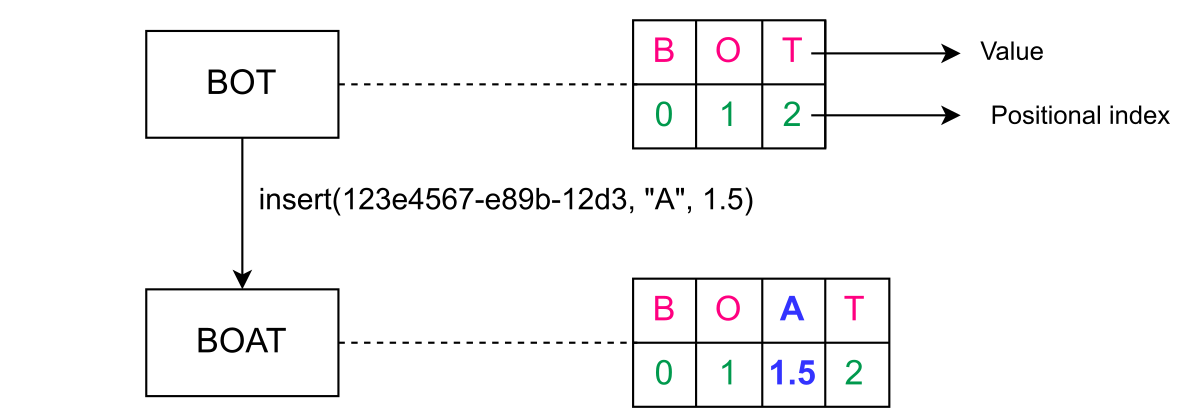
\includegraphics[width=0.5\textwidth]{Images/chapter_38/section_6200295243120640/4842605069729792.png}
 \caption{Preventing order dependency between operations}
\end{figure}

CRDTs ensure strong consistency between users. Even if some users are offline, the local replicas at end users will converge when they come back online.
\\
Although well-known online editing platforms like Google Docs, Etherpad, and Firepad use OT, CRDTs have made concurrency and consistency in collaborative document editing easy. In fact, with CRDTs, it's possible to implement a serverless peer-to-peer collaborative document editing service.
\begin{quote}
\textbf{Note:} OT and CRDTs are good solutions for conflict resolution in collaborative editing, but our use of WebSockets makes it possible to highlight a collaborator's cursor. Other users will anticipate the position of a collaborator's next operation and naturally avoid conflict.
\end{quote}

\begin{quote}
\textbf{Quiz:}
\textbf{Question 1:} Why can't we use locks to synchronize between users?
\textbf{Answer:} Locks require us to segment documents into small sections where users could lock a portion and edit it. This will help developers come up with an easy solution and avoid complexities like OT and CRDTs. However, this also leads to poor user experience. For example, two users may want to add characters to the same section of the document, but their operations may not necessarily conflict. A lock is a good choice for services like

Google Sheets. This is because the document is divided into equal sizes of small cells, and only one user can add or edit the contents of a specific cell.
\textbf{Question 2:} What happens if there are two users collaborating on a document and they have different Internet speeds? Which technology, OT or CRDT, is better suited for conflict resolution in such a case?
\textbf{Answer:} With a varied Internet connection speed, the order of operations between users can lead to problems. However, operations are order dependent in

OT, whereas operations in CRDTs are order independent. This is why CRDTs are a suitable solution to such a problem.
\end{quote}

% End of section content